%===================================== CHAP 6 =================================
\chapter{Experimental Setup}\label{chapter_experimental_setup}



\section{Data}
For this thesis we have mainly used FPL data provided by fantasyoverlord.com. Fantasy overlord contains detailed gameweek data for both the 2016/2017- and the 2017/2018 season. Further, clubelo.com has been used in order to obtain ELO values for each Premier League team. In addition, Sportradar has provided odds and probabilities for the fixtures of the 2017/2018 season. 
\newpar
The model presented in chapter \ref{chapter_model_formulation} has been run for the first 35 gameweeks of the 2017/2018 season. Ideally, the model should be run for the entire season. However, due to the deadline of the thesis this was not possible. 

\subsection{Processing of player data}
\subsubsection{Injuries and suspensions}
Once a player is listed as injured and thus unavailable for the upcoming gameweek, it is reasonable to set his expected points to zero. In order to account for injury status, we created a matrix of 0's and 1's. Fit players are assigned with a value of 1, while injured players are assigned with a value of 0. By multiplying each player's expected points by this injury matrix, injured players' expected points are automatically set to zero. As it is difficult to decide exactly when an injured player will be fit again, it is assumed in the solution approach that once a player is listed as injured, he will be unavailable for all upcoming  gameweeks. However, the injury list is updated for each gameweek, hence a player's injury status might change after a gameweek has been played. During the season we have collected injury data from fantasypremierleague.com ahead of each gameweek. Players that were listed with a 0\% probability of playing were listed as injured for the upcoming gameweek. 
\newpar
In addition, the model accounts for suspensions when optimizing the team for a gameweek. A player may be suspended for up to three games when receiving a red card, depending on whether it was a direct red card or not. Further, a player is subject to a match ban if he receives his 5th, 10th or 15th yellow card of the season. In addition, a player can be suspended by the English Football Association if he is found guilty of unsportsmanlike conduct. As for the injuries, a player that is suspended is rewarded with an expected points of 0 in the gameweeks of his suspensions. 

\subsubsection{Promoted teams}
Gathering data for newly promoted teams is rather difficult, as this data is not easy obtainable. In addition, it requires a lot of computational work in order to compare performances in the English Championship to the Premier League. Due to these difficulties, some simplifications are made. In general, players on newly promoted teams are not considered in the first gameweek of the 2017/2018 season. However, if a player was transferred to a promoted team ahead of the season, and he played in the Premier League in the previous season, the player would then be included from the start of the season. It is worth noticing that the newly promoted teams are partly considered in the first gameweek when using the average method. This is solved by using the ELO system. 
\subsubsection{Players transferred ahead of 2017/2018 season}
A question that arise with the international transfer window, is how new players is going to perform in another league in a different country. Forecasts of these players performance could be obtained by studying their performance from previous seasons in their respective leagues and hence somehow compare a performance in a different league with a performance in Premier League. However, it is very difficult to compare one league to another. Further, it must be done for several leagues, for instance the Spanish La Liga, the Italian Serie A, the German Bundesliga, the Dutch Eredivisie etc. For simplicity, this type of work is not considered in this thesis.
\newpar
In this project it is assumed that the creators of Fantasy Premier League have assigned new players with a price that is perfectly mirrored by their expected performance. Thus, one can compare the new players with existing FPL players of the same price. For instance, if a new midfielder is listed with a price of 9, it is assumed that this player will have the same expected performance as other midfielders listed with the same price.
\subsubsection{Irregular gameweeks}
In general, every gameweek consists of 10 fixtures featuring every team once. However, due to matches in the national and international cups, some of the Premier League matches are postponed or played ahead of the original date. This implies that some of the gameweeks do not consist of exactly 10 fixtures, but perhaps 8 or 12 for instance. Thus, in these gameweeks some players may be featured twice, gaining points for both matches. Similarly, some players will not be featured in other gameweeks, these gameweeks are hereby referred to as \textit{blanks}.

\section{Forecasting Error}

The forecasting error of the complete 2017/2018 season based on the two average-based models are summarized in Table \ref{tab:accuracy_average}. Note, however, that it is not given that the method with lowest error will performed best. 

\begin{table}[H]
\centering
\caption{Summary of forecasting errors on the average methods}
\label{tab:accuracy_average}
\begin{tabular}{llll}
Method & ME & RMSE & MAE\\
Argentina & 0.00882 & 2.436 & 1.295 \\
Improved  & 0.0436  & 2.455 & 1.294 \\ 
Odds  & NA  & NA & NA   \\
Regression  & NA  & NA & NA \\
\end{tabular}
\end{table}

\section{Setting Parameters}
veldig viktig diskusjon: 
at vi har forstått at det er feil å sette høye penalties, men at vi er ute etter å få en modell som presterer bra. 


\subsection{Modified Average}
In this thesis, the relative team strength factors are calculated according to the Elo values provided by clubelo.com. As the Elo values are updated for every gameweek, each Premier League team is assigned with 38 different Elo values, depending on the results in their previous games. An overview of the Elo values is attached in the appendix. 
\newpar
Table \ref{Field advantage} provides the calculated values for field advantages for the past five Premier League seasons. As observed, the field advantages are somewhat constant, with the home field advantage ranging from 1.105 to 1.149 and the away field advantage ranging from 0.851 to 0.895. Hence, simply taking the average over the past five years seems to yield an appropriate field advantage factor. 

\begin{table}[H]
\centering
\smaller
\caption{Field advantages for previous 6 seasons}

\begin{tabular}{|l|l|l|l|l|l|l|l|l|}
\hline
          & 16-17    & 15-16    & 14-15    & 13-14    & 12-13 & 11-12 & \textbf{17-18 Avg} & \textbf{16-17 Avg}  \\
          \hline
        
Home advantage & 1.141 & 1.105 & 1.149 & 1.137 & 1.114 & 1.133 & \textbf{1.129} & \textbf{1.128} \\
\hline
Away advantage & 0.859 & 0.895 & 0.851 & 0.863 & 0.886 & 0.867 & \textbf{0.871} & \textbf{0.872} \\
\hline
\end{tabular}
\label{Field advantage}
\end{table}




As for the point streak factor, the variables X and Y has to be decided. As goalkeepers and defenders receive 4 points for keeping a clean sheet, all players get 3 points for an assist and midfielders and forwards get 5 and 4 points respectively for scoring a goal, the X variable should be set according to these numbers. Further, as a player gets 2 points for playing more than 60 minutes, it is appropriate to let the X variable take a value of 5. Hence, if a player keeps has an assist or scores a goal and in addition plays 60 minutes or more, he will receive enough points to be on a positive point streak given that he did not receive a yellow or red card. As for the Y variable, a player that does not contribute with neither a goal, assist nor a clean sheet is awarded maximum 2 points. Thus, it is reasonable to set the Y to equal 2 points. 
\subsubsection{Determining optimal forecasting horizon, optimization horizon and penalty term}

In a case with perfect information available, the optimal optimization horizon is the complete season of 38 gameweeks. Furthermore, the penalty term would be 4, as stated in the rules of the game. However, we do not operate within the domain of perfect information, so these parameter settings are not guaranteed optimal. Further, decisions must be made on how many matches to look back in the past when calculating the forecasts based on average performance in previous games.
\newpar 
In order to set the values of the parameters in a sensible way, a number of different combinations of the three parameters are run on the 2016/2017 season. Figure \ref{Parameter_choice} provides an overview of how the mean value of points for the entire 2016/2017 season changes with different forecasting horizons, optimization horizons and penalty terms. In the figure, only the best run (maximum mean) for each different penalty value from 3-20 is plotted. One should be careful not to make to categorical statements based on the figure. However, some insights can be reached. First, an optimization horizon of 3-4 appears to  be ideal. It is important to stress that each combination of optimization and forecast horizon are run as long as the optimization horizon is not greater that the forecast horizon. However, in the model, maximum only occurs for horizons from 1-4, and the by far best results are 3 or 4. Furthermore, a penalty in the range of 15-20 appears to yield the best results. As does a forecasting horizon between 5-6. However, this is not unexpected. When the forecast horizon is 6 weeks, we can only consider the matches after gameweek 6 has been played. Hence, we get an opportunity of initially selecting the players that have performed best over the 6 first gameweeks. Intuitively, the results will be better as the forecast horizon increases, as one get the opportunity of initially selecting players that have already proven to perform well the same season. Table \ref{tab:top_10} displays the 10 best combinations. The table clearly shows that a penalty between 15-20, optimization horizon of 3-4 and forecast horizon of 5-6 was optimal in the 2016/2017 season, when mean is considered. Again, we stress that the intuitively is expected to increase with a longer forecast horizon. Table \ref{tab:top_5} displays the best combinations when forecasting horizon is held fixed forecasting horizon. Figure \ref{fig:fixed_f_hor} displays the best combinations with a fixed forecasting horizon.

\begin{figure}[H]
    \centering
    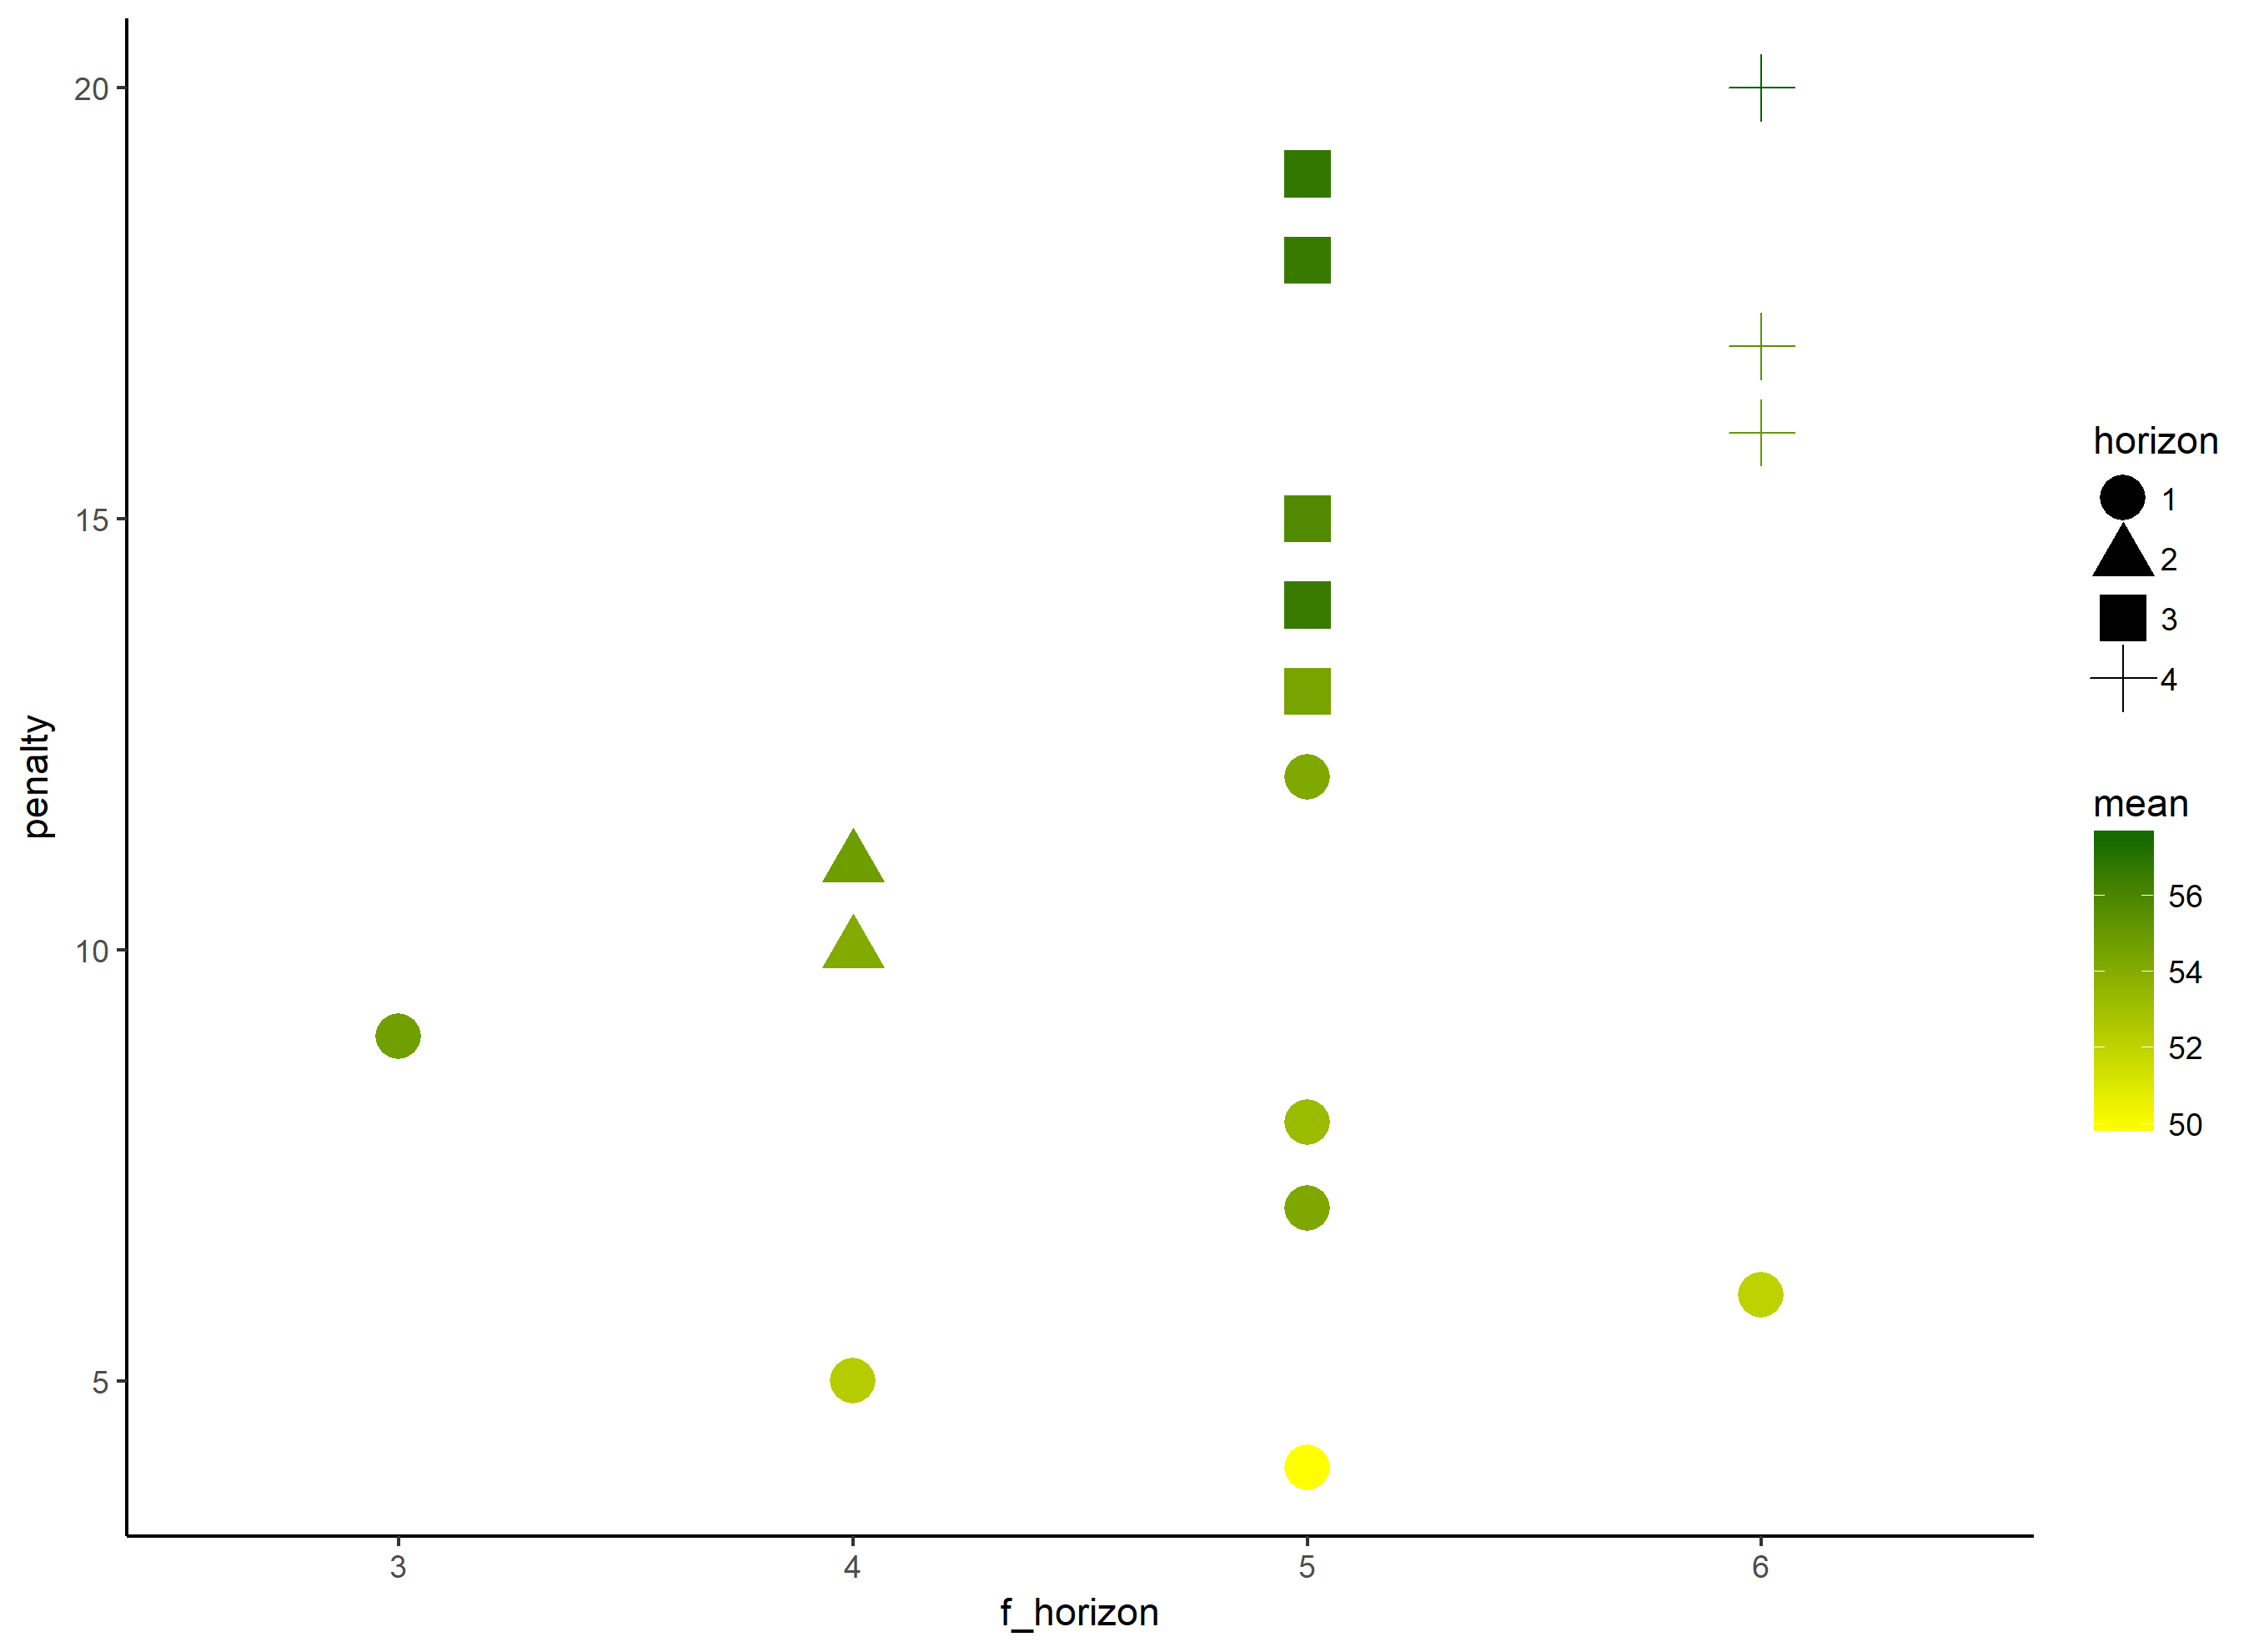
\includegraphics[scale=0.55]{fig/chapter_6/paramter_choice.png}
    \caption{Performance with different transfer penalties, optimization horizons and forecast horizons}
\label{Parameter_choice}    
\end{figure}

\begin{table}[H]
\centering
\caption{The 10 best combinations of parameters}
\label{tab:top_10}
\begin{tabular}{lllll}
Penalty & Horizon & Forecast Horizon & Total Points & Mean  \\
20      & 4       & 6                & 1851         & 57.84 \\
20      & 4       & 5                & 1899         & 57.55 \\
19      & 3       & 5                & 1875         & 56.82 \\
18      & 3       & 5                & 1869         & 56.64 \\
14      & 3       & 5                & 1868         & 56.61 \\
18      & 4       & 6                & 1808         & 56.50 \\
19      & 4       & 6                & 1806         & 56.44 \\
20      & 3       & 5                & 1860         & 56.36 \\
20      & 5       & 5                & 1851         & 56.09 \\
18      & 6       & 6                & 1793         & 56.03
\end{tabular}
\end{table}

\begin{table}[H]
\centering
\caption{The best combinations for each forecast horizon}
\label{tab:top_5}
\begin{tabular}{lllll}
Penalty & Horizon & Forecast Horizon & Total Points & Mean  \\
9       & 1       & 3                & 1914         & 54.69 \\
11      & 2       & 4                & 1863         & 54.79 \\
20      & 4       & 5                & 1899         & 57.55 \\
20      & 4       & 6                & 1851         & 57.84
\end{tabular}
\end{table}

\begin{figure}[H]
    \centering
    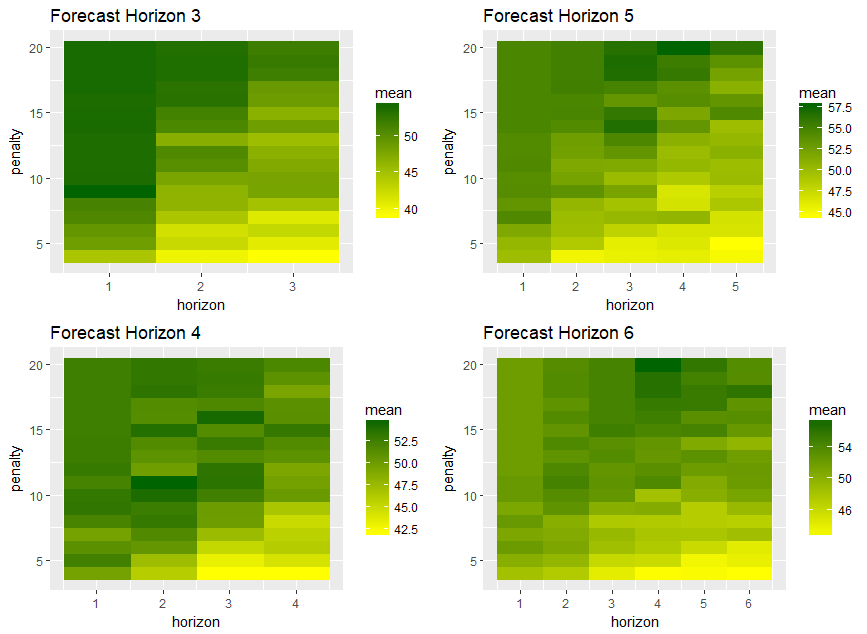
\includegraphics[scale=0.55]{fig/chapter_6/parameter_choice_fixed_f_hor.png}
    \caption{Performance with different transfer penalties and optimization horizons, but fixed forecast horizon}
\label{fig:fixed_f_hor}    
\end{figure}

\begin{comment}
In general, one can see that low transfer penalties combined with a high forecast horizon yield the poorest results. Furthermore, it seems like choosing 7 or 8 as the forecast horizon is the wiser choice. In addition, the transfer penalty should be set to a value above 10. Based on figure \ref{Parameter_choice}, a combination found in the center appears to be optimal, and the values $h = 6$, $f = 7$ and $p = 11$ are chosen. Also, a combination of $h = 4$, $f = 8$ and $p = 14$ yield good results. 
\newpar

\end{comment}

\begin{comment}

\subsubsection{Forecast Horizon 3}

\begin{figure}[H]
    \centering
    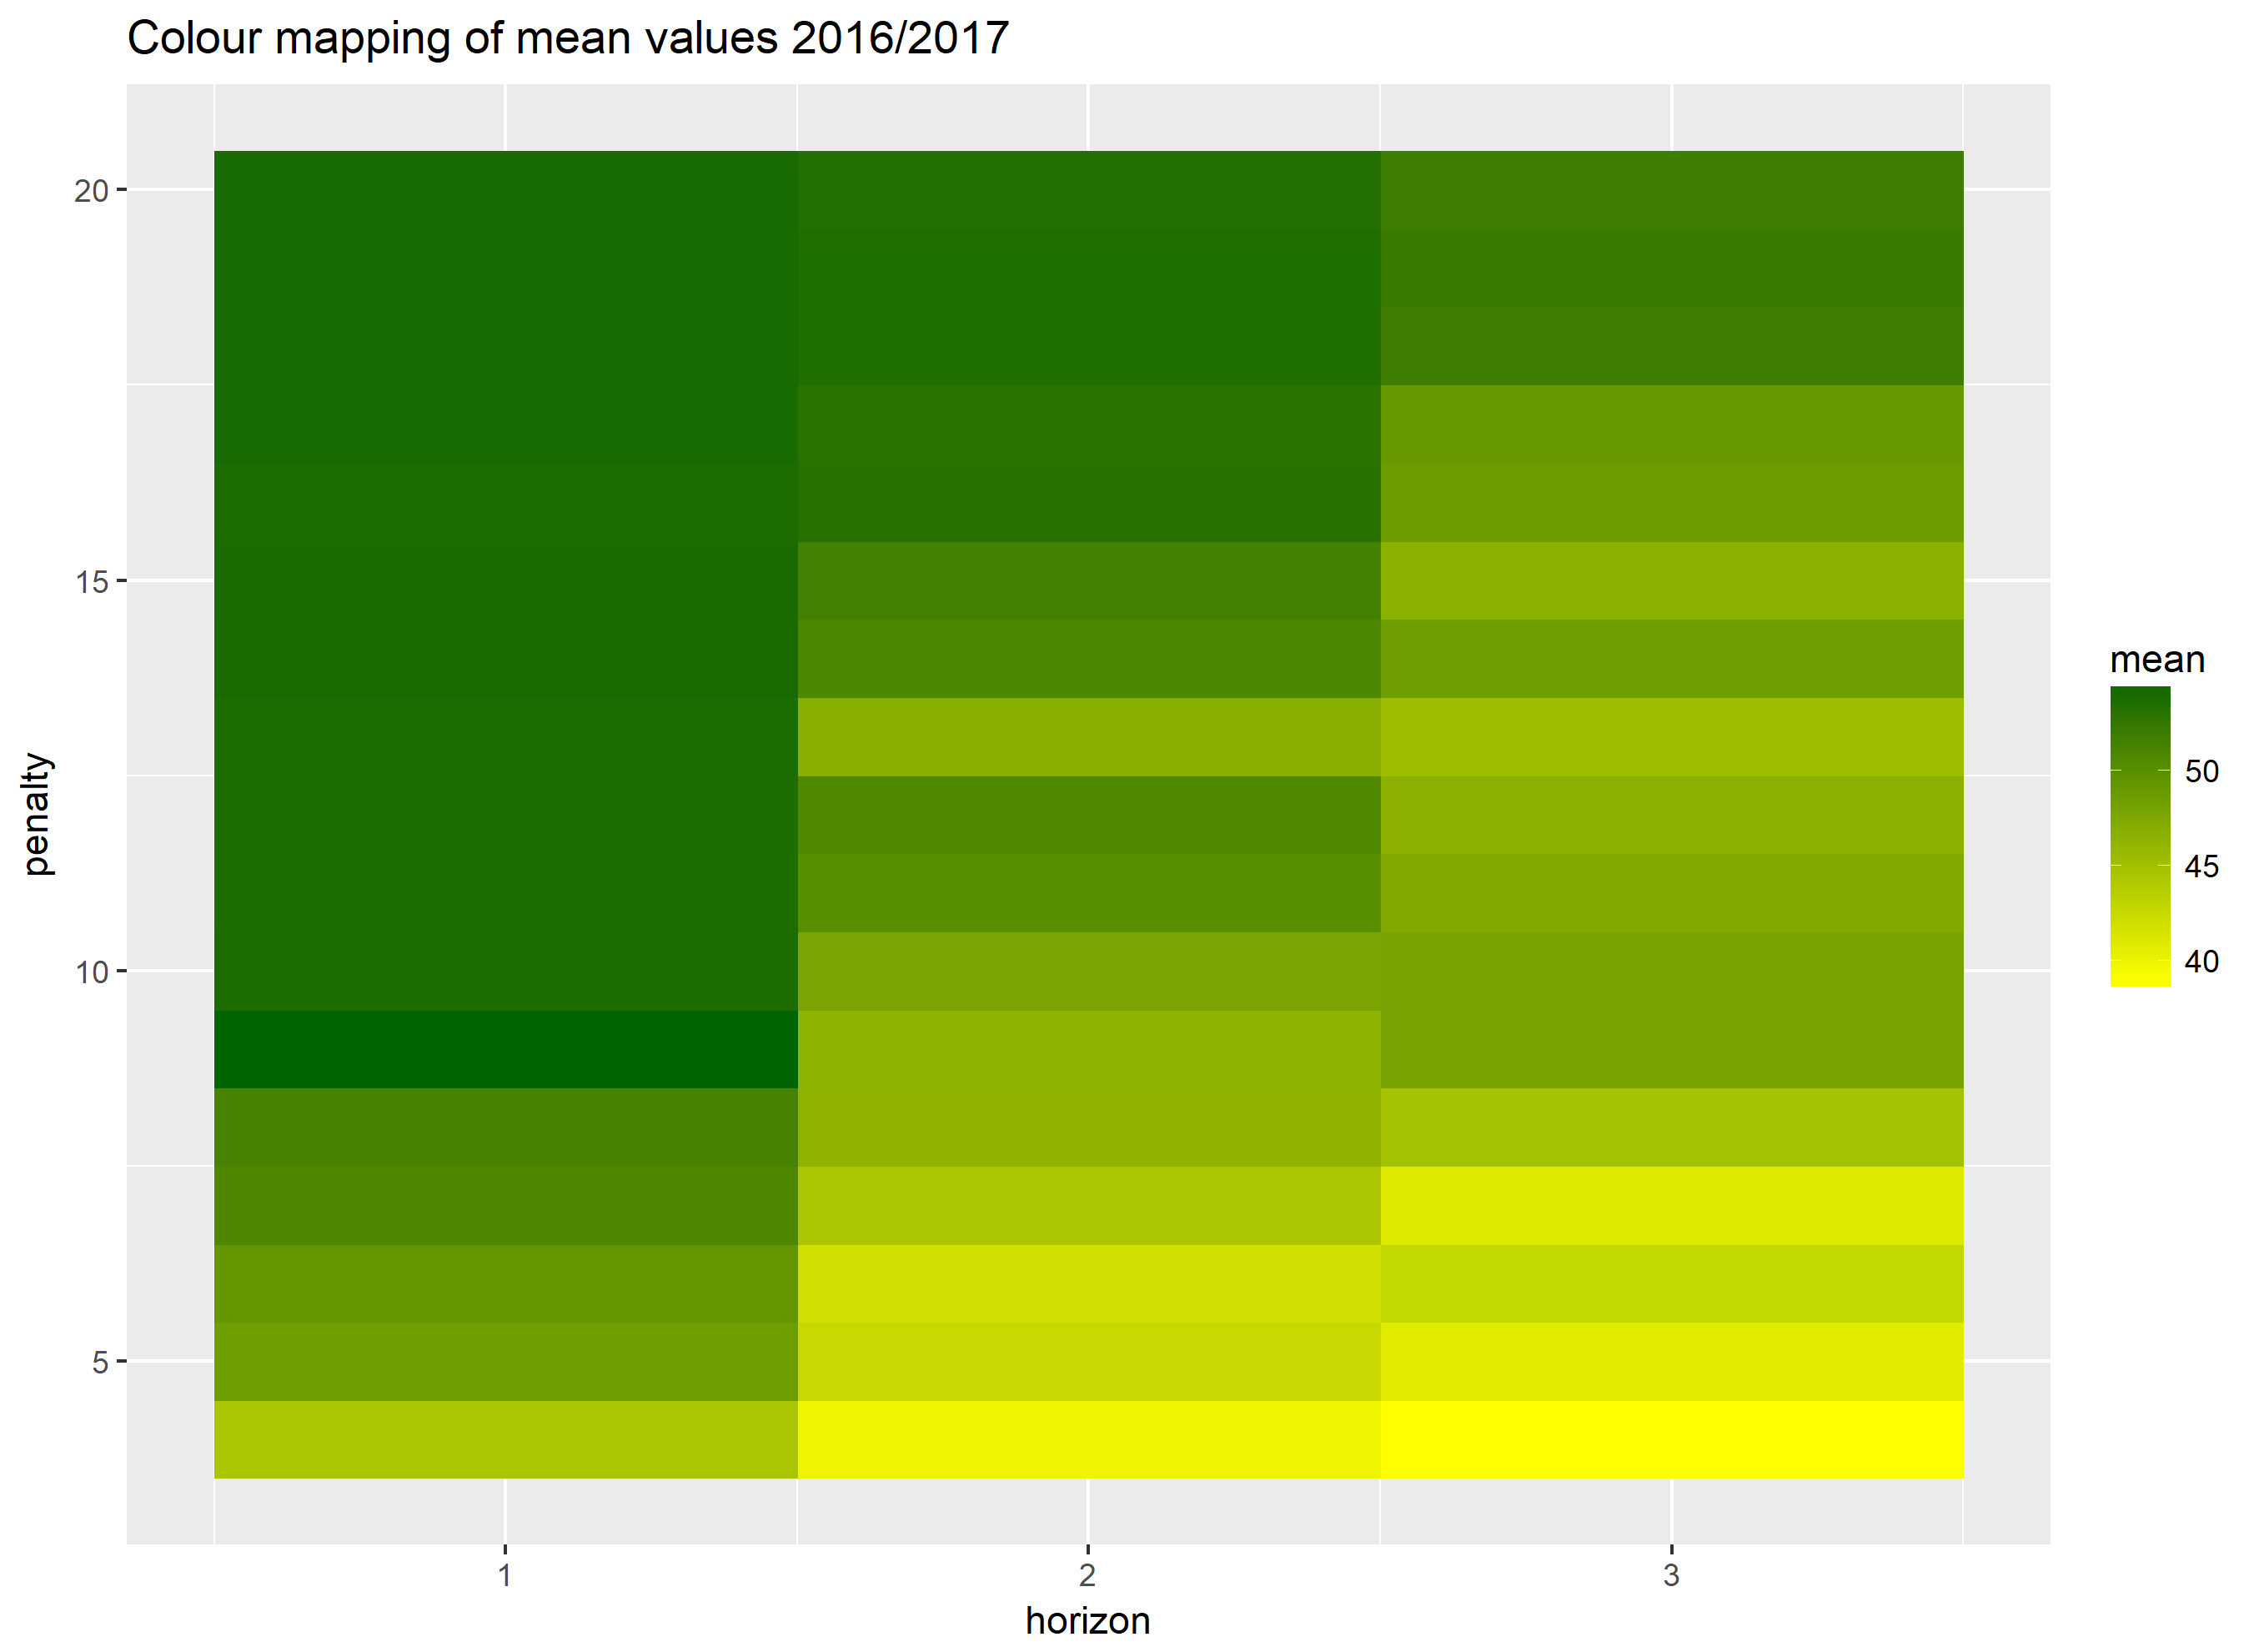
\includegraphics[scale=0.55]{fig/chapter_6/paramter_choice_3.png}
    \caption{Overview of total score with forecast horizon 3}
\label{fig:parameters_f_hor_3}    
\end{figure}

\subsubsection{Forecast Horizon 4}

\begin{figure}[H]
    \centering
    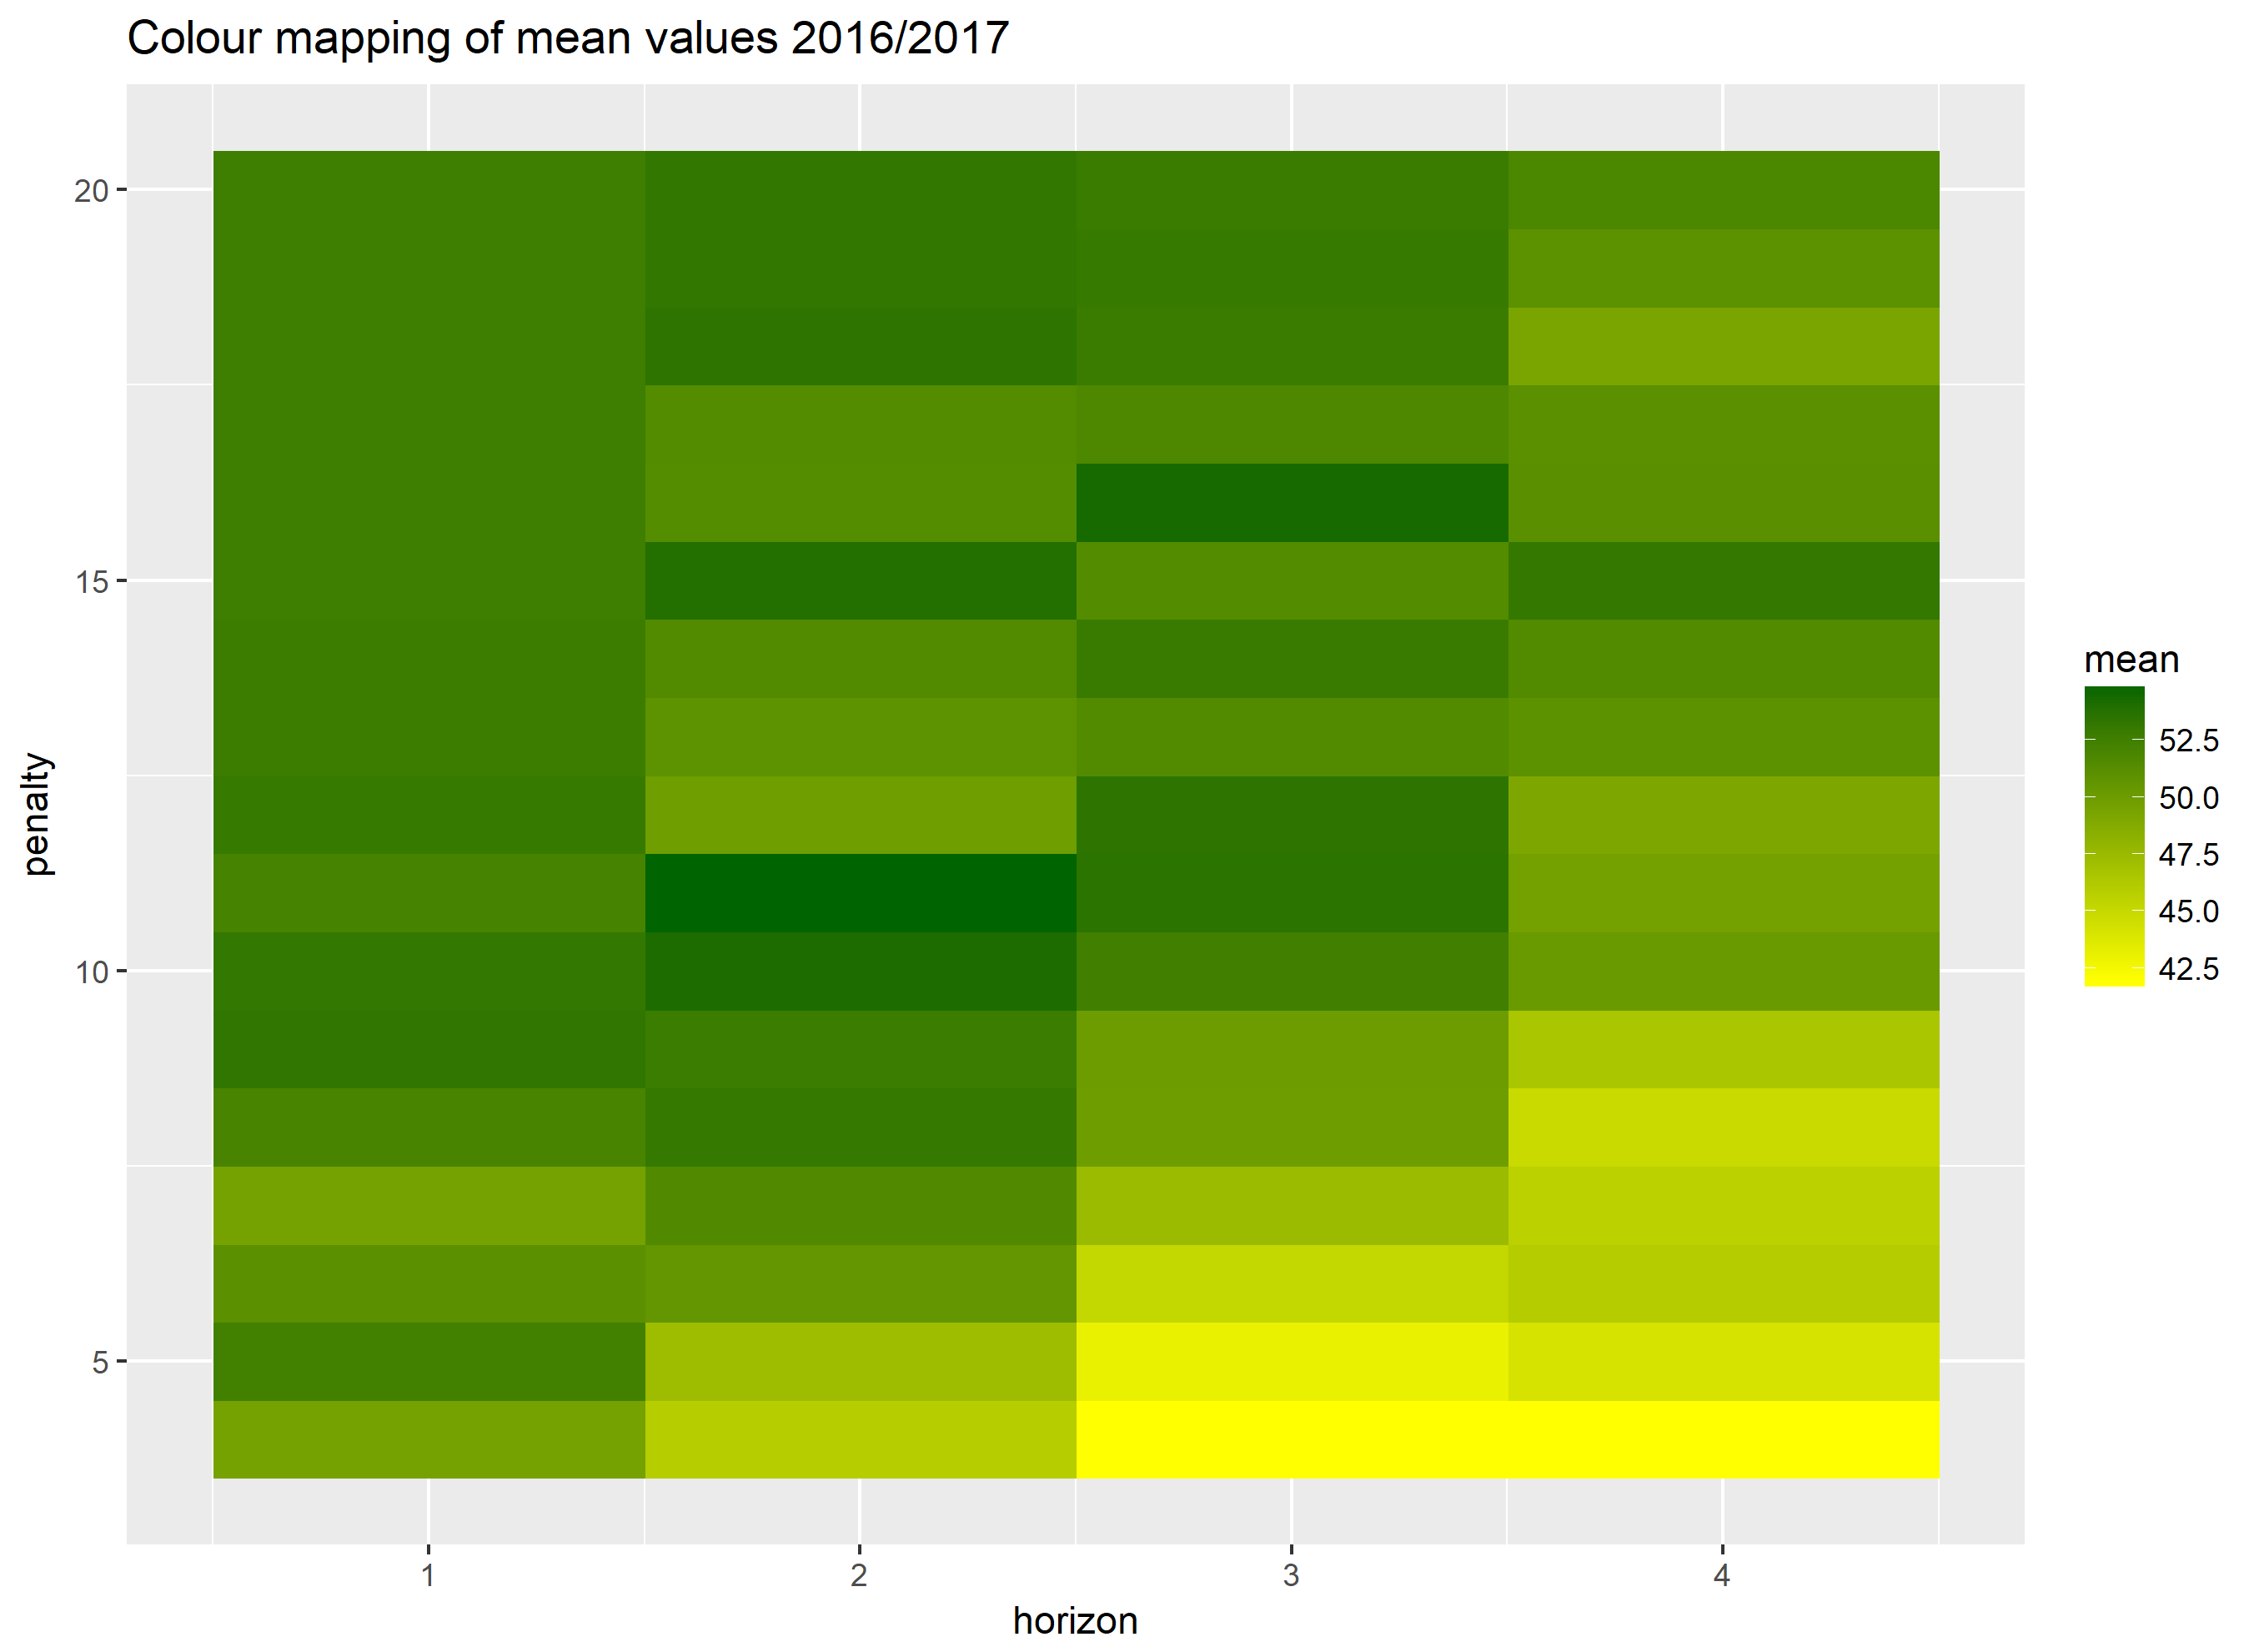
\includegraphics[scale=0.55]{fig/chapter_6/paramter_choice_4.png}
    \caption{Overview of total score with forecast horizon 4}
\label{fig:parameters_f_hor_4}    
\end{figure}

\subsubsection{Forecast Horizon 5}

\begin{figure}[H]
    \centering
    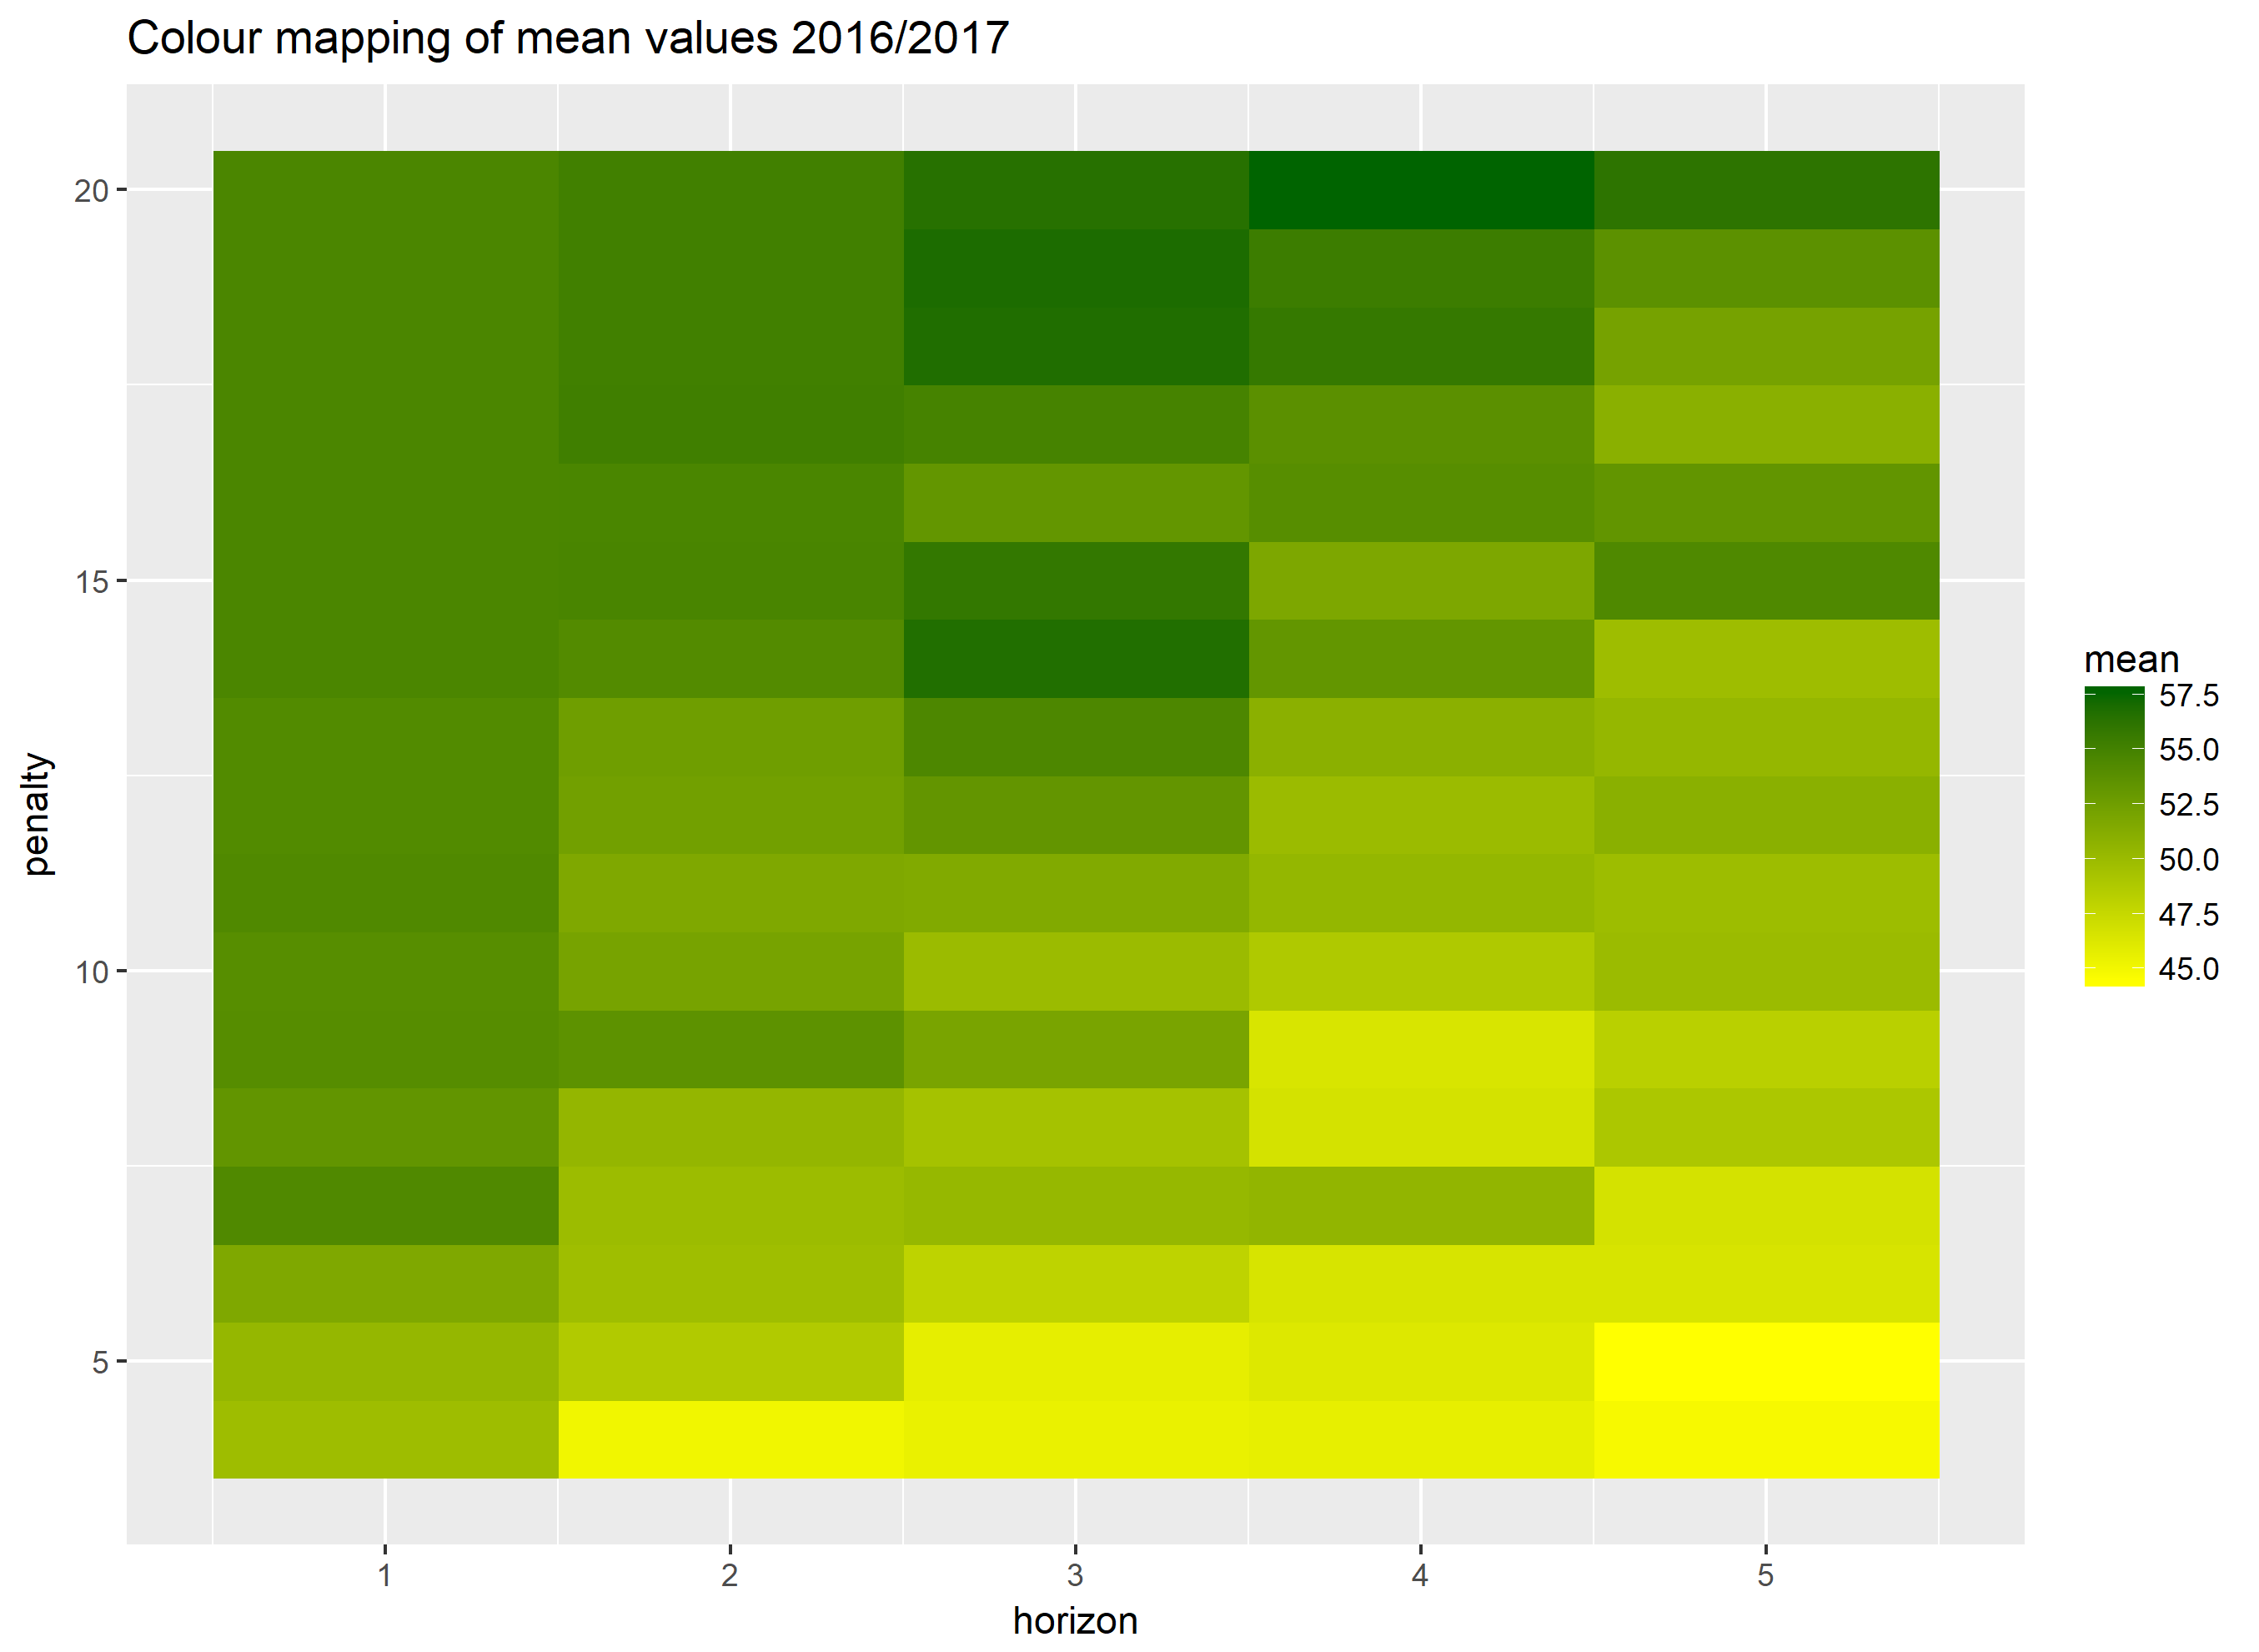
\includegraphics[scale=0.55]{fig/chapter_6/paramter_choice_5.png}
    \caption{Overview of total score with forecast horizon 5}
\label{fig:parameters_f_hor_5}    
\end{figure}

\subsubsection{Forecast Horizon 6}

\begin{figure}[H]
    \centering
    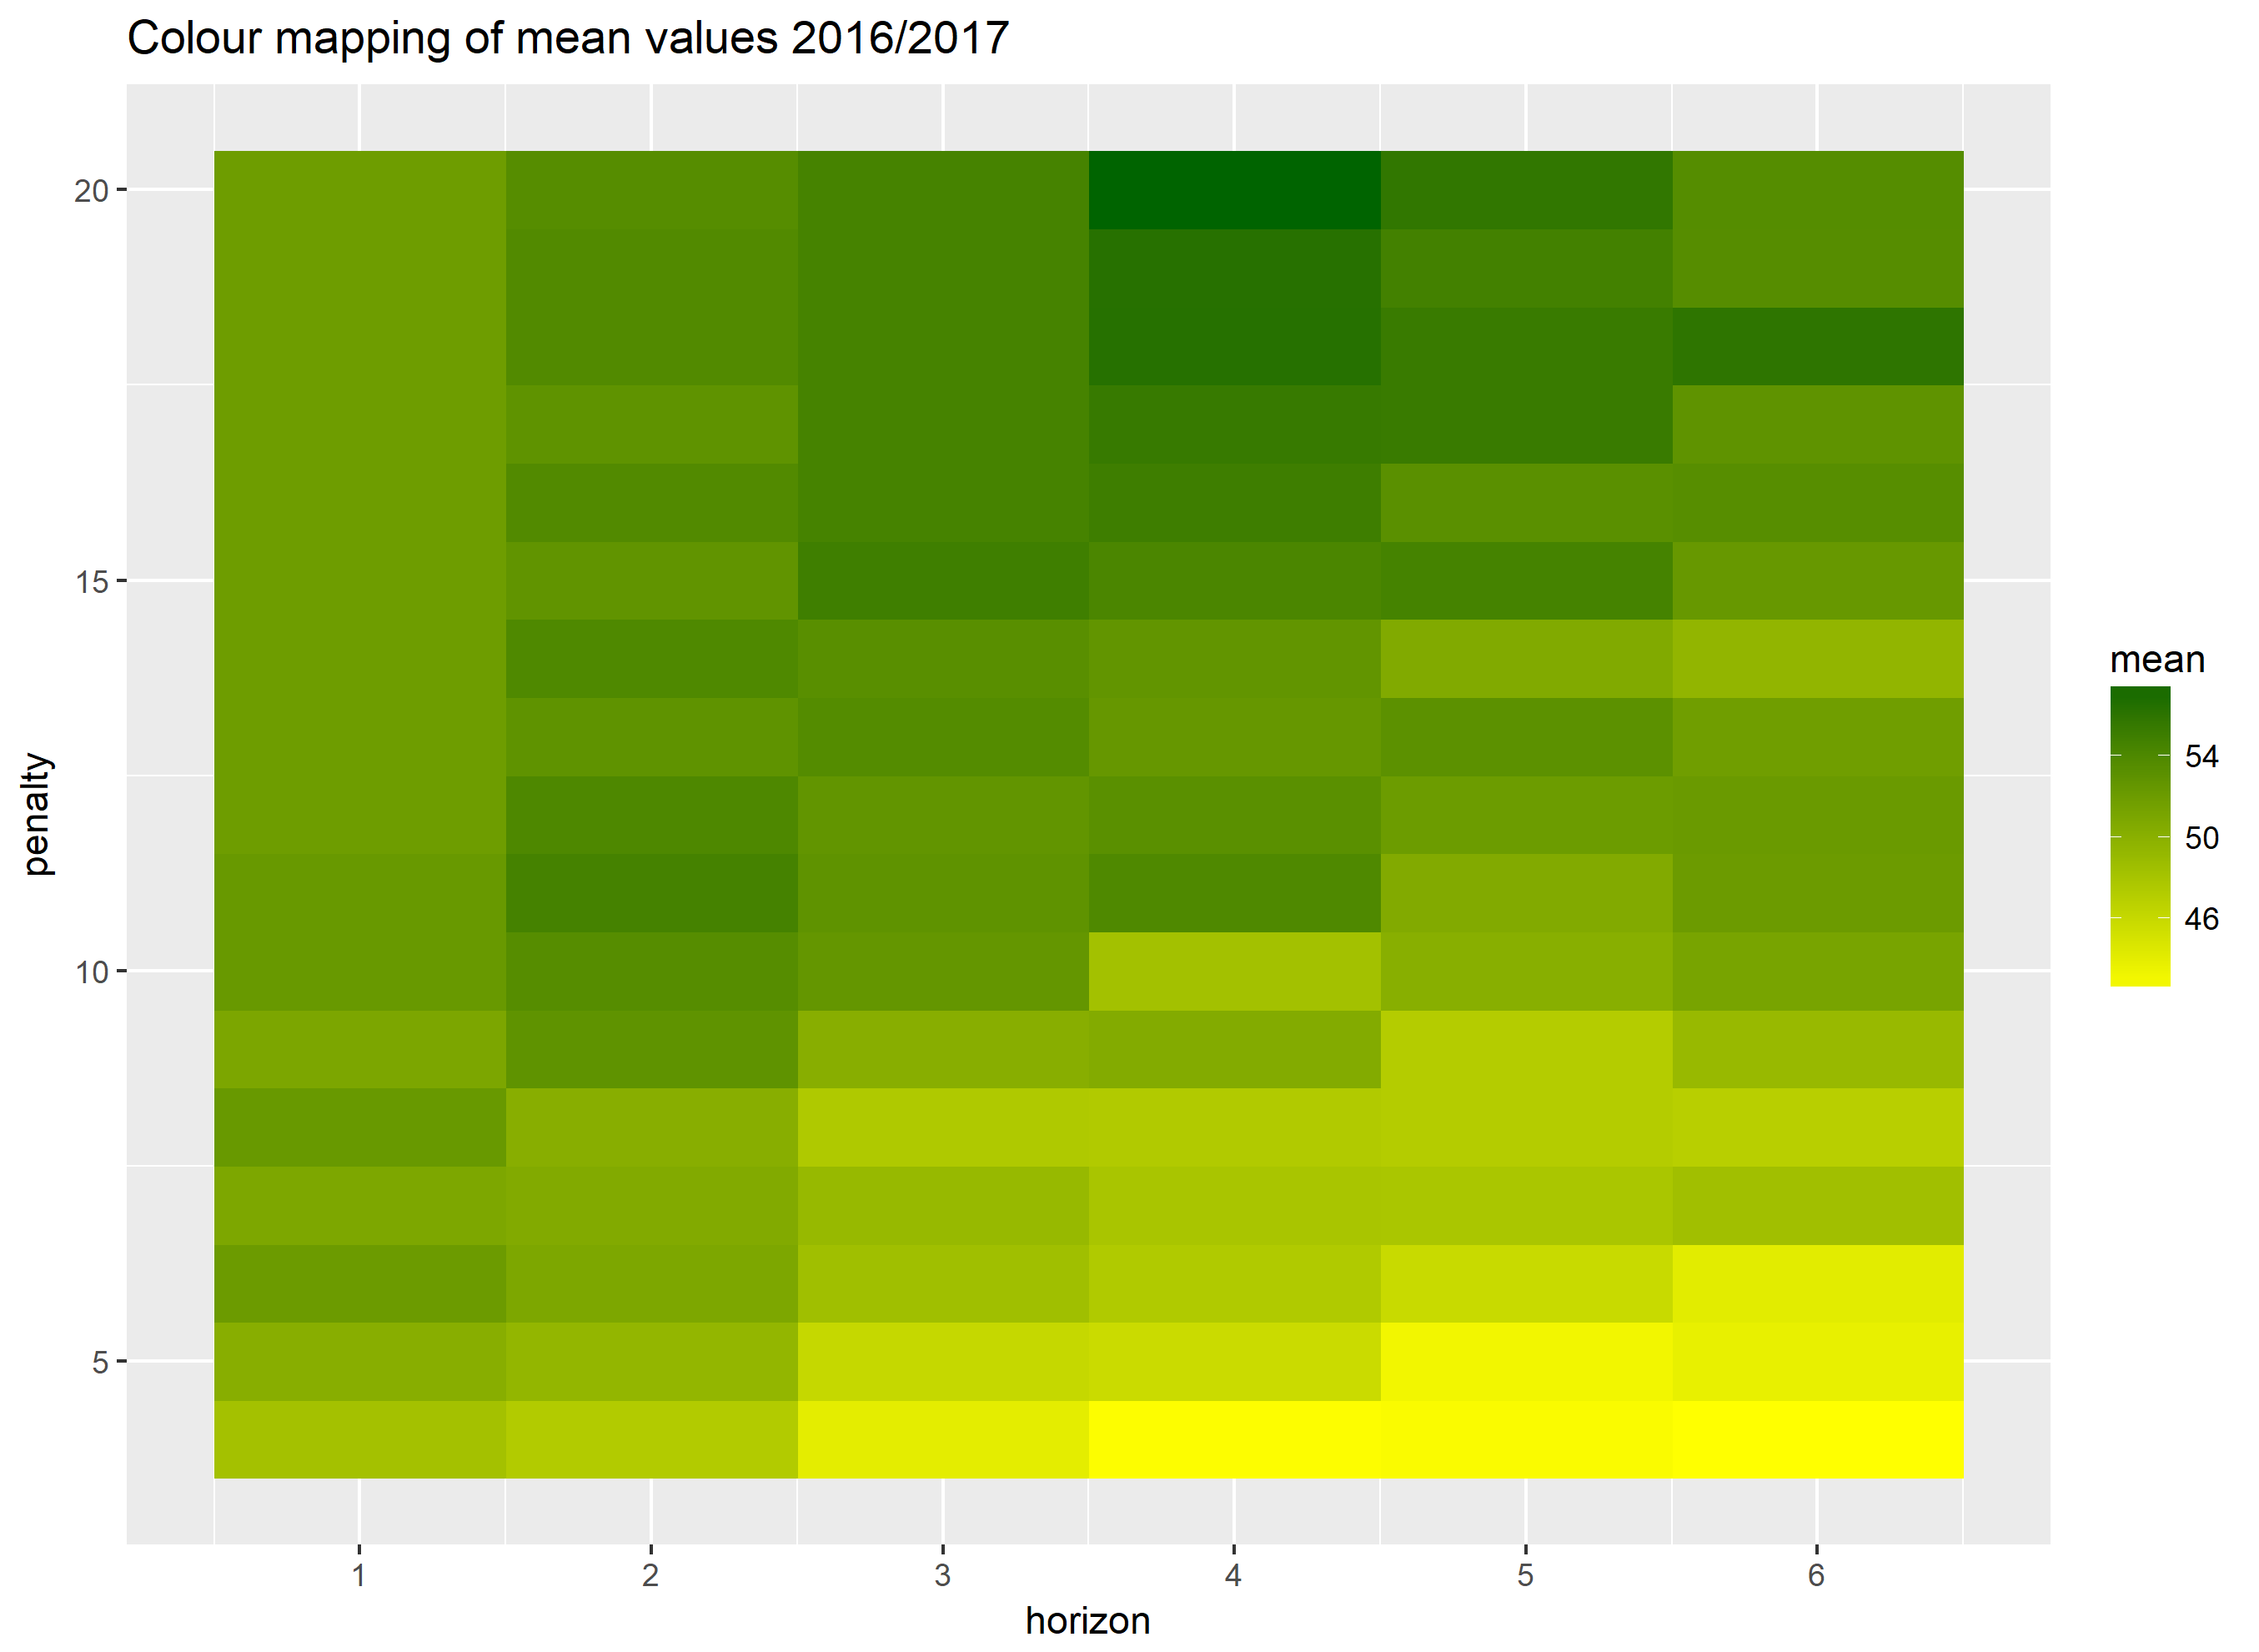
\includegraphics[scale=0.55]{fig/chapter_6/paramter_choice_6.png}
    \caption{Overview of total score with forecast horizon 6}
\label{fig:parameters_f_hor_6}    
\end{figure}

\end{comment}

Table \ref{tab:top_10} shows that a forecast horizon of 6 gameweeks combined with a optimization horizon of 4 gameweeks and a transfer penalty of 20 yields the highest mean for the 2016/2017 season. However, the next 4 top means are achieved with a forecast horizon of 5 gameweeks. Considering this, combined with the fact that an increasing forecast horizon limits the amount of gameweeks considered, we find it appropriate to select 5 gameweeks as the optimal forecast horizon. Moreover, according to table \ref{tab:top_10} an optimization horizon of 3 or 4 gameweeks is optimal. For high penalties, this is confirmed by figure \ref{fig:fixed_f_hor}. Furthermore, the figure illustrates that the optimization horizon of 6 gameweeks yields the highest mean for a forecast horizon of 5 gameweeks. However, it can be observed that an optimization horizon of 3 gameweeks in general performs better than that of 4 gameweeks. Therefore, we find it convenient to set the optimization horizon to 3 gameweeks when applying the adjusted average approach for the 2017/2018 season. Finally, figure \ref{fig:fixed_f_hor} illustrates that a higher penalty yields better means for the 2016/2017, reaching its best performance for penalties ranging from 14 to 20. As the results are somehow inbetween these penalties and dependent on the choices of the forecast- and optimization horizon, we have chosen a penalty value of 16. 

\subsection{Regression}

\subsubsection{Position Clustering}

Here, a rational for the clustering might appear.

\subsubsection{Time Series of Points}

In order to determine if one should view the points a player obtains as a time series, or is just as well off by only looking at aggregated numbers, the Durbin-Watson and Ljung-Box test for autocorrelation are performed. In Table \ref{tab:auto_tests} the results of the Durbin-Watson test and Ljung-Box test with lags from 1-5 are presented. Based on the results, 75\%-95\% of the players appear to have insignificant autocorrelation in their time-series of points. This result should be interpreted carefully. For instance, the players that did not play the entire season earned 0 points in each gameweek, and would certainly exhibit no autocorrelation. Regardless, it might be valuable to treat aggregates only, and neglect the effect time-series effects in the regression. The methodology works as a fine complement to the average method, where the points in latest games only is considered.

\begin{table}[H]
\centering
\caption{Summary of percentage of players with insignificant autocorrelation for different tests}
\label{tab:auto_tests}
\begin{tabular}{ll}
Test            & \% of players with insignificant autocorrelation \\
Durbin-Watson   & 94 \%                                            \\
Ljung-Box lag 1 & 76 \%                                            \\
Ljung-Box lag 2 & 76 \%                                            \\
Ljung-Box lag 3 & 78 \%                                            \\
Ljung-Box lag 4 & 80 \%                                            \\
Ljung-Box lag 5 & 81 \%                                           
\end{tabular}
\end{table}

\subsubsection{Variable Selection}

As described in the Solution approach outlined in Chapter 5, lasso regression is performed in order to determine the variable selection. 80\% of the data of the 2016/2017 season is used for training, and the remaining 20 \% for testing. In the following, the variables deemed significant alongside a plot or RMSE against values of log($\lambda$) for each position is presented.\newpar


In Figures \ref{fig:lasso_GLK_1}, \ref{fig:lasso_DEF_1}, \ref{fig:lasso_MID_1} and \ref{fig:lasso_FWD_1} the RMSE of the test set is plotted against different values of $\lambda$ for goalkeepers, defenders, midfielders and forwards respectively. Further, their significant variables are listed in tables \ref{tab:sig_var_GLK_1}, \ref{tab:sig_var_DEF_1}, \ref{tab:sig_var_MID_1} and \ref{tab:sig_var_FWD_1} respectively.

\begin{comment}


\begin{figure}[H]
    \centering
    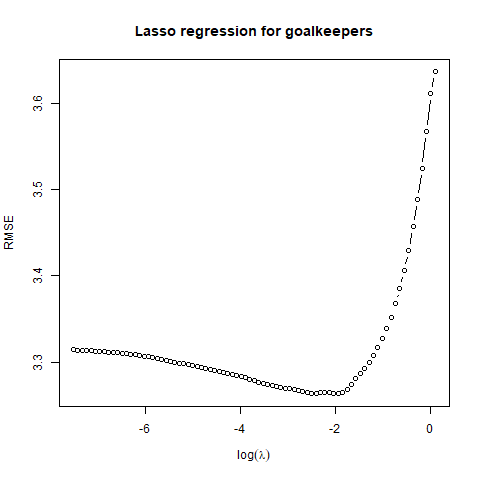
\includegraphics[scale=0.55]{fig/chapter_6/lasso_GLK.png}
    \caption{RMSE for different values of $\lambda$ for goalkeepers}
\label{fig:lasso_GLK}    
\end{figure}


\begin{table}[H]
\centering
\caption{Significant Variables for goalkeepers based on lasso regression and RMSE}
\label{tab:sig_var_GLK}
\begin{tabular}{l}
\textbf{Significant variables for goalkeepers }\\
Opponent                              \\
Team                                  \\
Cost                                  \\
Transfers in                          \\
Transfers out                         \\
Home/Away                             \\
Minutes played                        \\
Saves                                 \\
Clean Sheets                          \\
Assists                               \\
Own Goals                            
\end{tabular}
\end{table}

\end{comment}


\begin{table}[H]
\centering
\begin{minipage}{.5\textwidth}
  \centering
  \captionsetup{justification=centering}
    \begin{figure}[H]
        \centering
        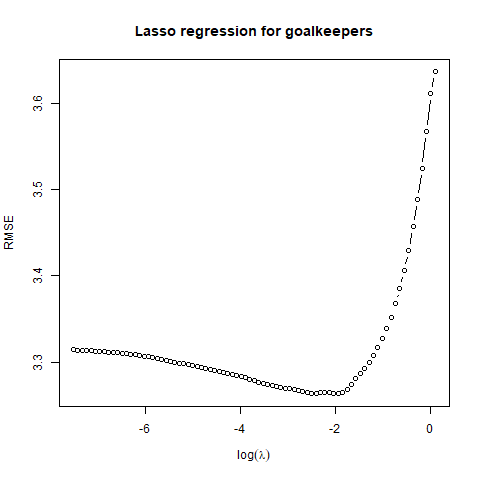
\includegraphics[scale=0.4]{fig/chapter_6/lasso_GLK.png}
    \end{figure}
    \captionof{figure}{RMSE for different values of $\lambda$ for goalkeepers}
    \label{fig:lasso_GLK_1}
\end{minipage}%
\begin{minipage}{.5\textwidth}
  \centering
  \captionsetup{justification=centering}
    \begin{tabular}{c}
    \\
    \textbf{Significant variables for Goalkeepers }\\
    \\
    \\
Opponent                              \\
Team                                  \\
Cost                                  \\
Transfers in                          \\
Transfers out                         \\
Home/Away                             \\
Minutes played                        \\
Saves                                 \\
Clean Sheets                          \\
Assists                               \\
Own Goals                            
    \\
    \\
    \\
    \\
\\


    \end{tabular}
\captionof{table}{Significant Variables for goalkeepers based on lasso regression and RMSE}
\label{tab:sig_var_GLK_1}
\end{minipage}
\end{table}

\begin{comment}
\textbf{Defenders}
In Figure \ref{fig:lasso_DEF} the RMSE of the test set is plotted against different values of $\lambda$. In Table \ref{tab:sig_var_DEF} the significant variables are listed
\end{comment}


\begin{table}[H]
\centering
\begin{minipage}{.5\textwidth}
  \centering
  \captionsetup{justification=centering}
    \begin{figure}[H]
        \centering
        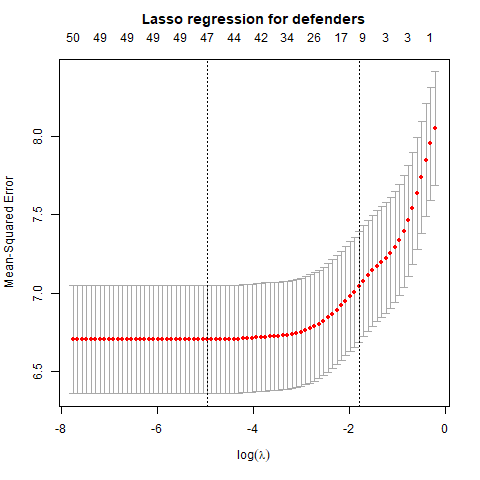
\includegraphics[scale=0.4]{fig/chapter_6/lasso_DEF.png}
    \end{figure}
    \captionof{figure}{RMSE for different values of $\lambda$ for defenders}
    \label{fig:lasso_DEF_1}
\end{minipage}%
\begin{minipage}{.5\textwidth}
  \centering
  \captionsetup{justification=centering}
    \begin{tabular}{c}
    \textbf{Significant variables for Defenders }\\
    \\
    \\
    \\
    
    Opponent                              \\
    Team                                  \\
    Cost                                  \\
    Transfers in                          \\
    Transfers out                         \\
    Home/Away                             \\
    Minutes played                        \\
    Yellow Cards                          \\
    Own Goals                             \\
    \\
    \\
    \\
    \\
   \\
   \\
    
    
    \end{tabular}
\captionof{table}{Significant Variables for midfielders based on lasso regression and RMSE}
\label{tab:sig_var_DEF_1}
\end{minipage}
\end{table}

\begin{comment}


\begin{figure}[H]
    \centering
    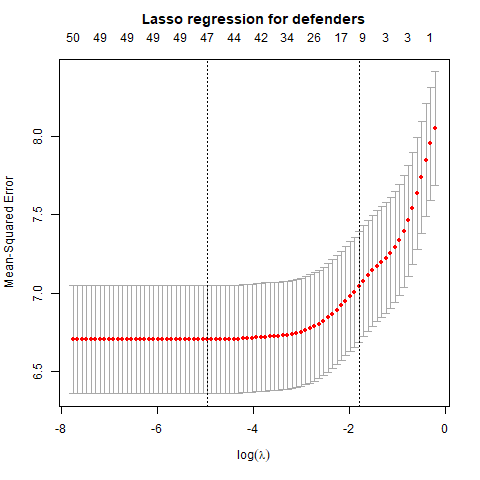
\includegraphics[scale=0.55]{fig/chapter_6/lasso_DEF.png}
    \caption{RMSE for different values of $\lambda$ for defenders}
\end{figure}

\begin{table}[H]
\centering
\caption{Significant Variables for defenders based on lasso regression and RMSE}
\begin{tabular}{l}
\textbf{Significant variables for Defenders }\\
Opponent                              \\
Team                                  \\
Cost                                  \\
Transfers in                          \\
Transfers out                         \\
Home/Away                             \\
Minutes played                        \\
Yellow Cards                          \\
Own Goals                                               
\end{tabular}
\end{table}

\end{comment}

\begin{comment}
\textbf{Midfielders}
In Figure \ref{fig:lasso_MID} the RMSE of the test set is plotted against different values of $\lambda$. In Table \ref{tab:sig_var_MID} the significant variables are listed
\end{comment}


\begin{table}[H]
\centering
\begin{minipage}{.5\textwidth}
  \centering
  \captionsetup{justification=centering}
    \begin{figure}[H]
        \centering
        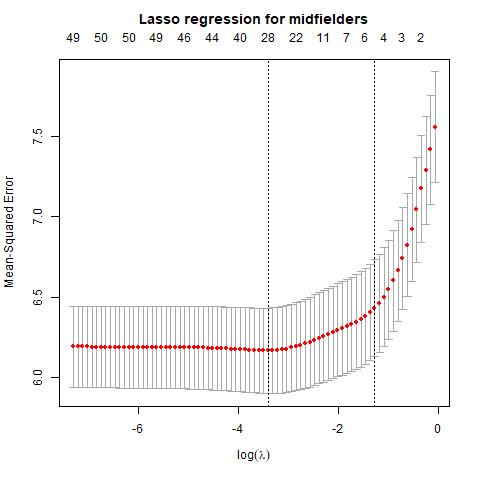
\includegraphics[scale=0.4]{fig/chapter_6/lasso_MID.png}
    \end{figure}
    \captionof{figure}{RMSE for different values of $\lambda$ for midfielders}
    \label{fig:lasso_MID_1}
\end{minipage}%
\begin{minipage}{.5\textwidth}
  \centering
  \captionsetup{justification=centering}
    \begin{tabular}{c}
    \\
    \textbf{Significant variables for Midfielders }\\
    \\
    \\
    \\
   Opponent                              \\
Team                                  \\
Cost                                  \\
Transfers in                          \\
Transfers out                         \\
Home/Away                             \\
Minutes played                        \\
Goals                                   \\
Penalty Misses                          \\
Clean Sheets                            \\
Assists                                 \\
\\
\\
\\

    \end{tabular}
\captionof{table}{Significant Variables for midfielders based on lasso regression and RMSE}
\label{tab:sig_var_MID_1}
\end{minipage}
\end{table}

\begin{comment}


\begin{figure}[H]
    \centering
    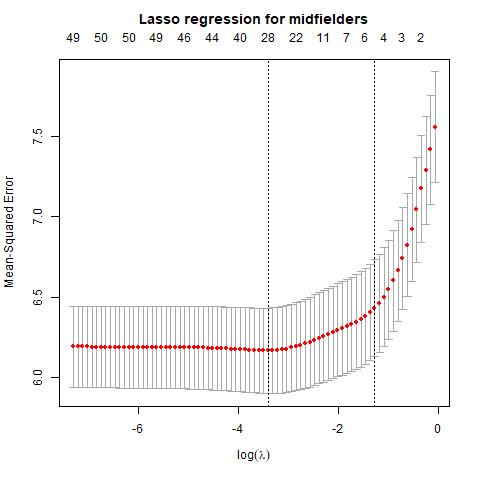
\includegraphics[scale=0.55]{fig/chapter_6/lasso_MID.png}
    \caption{RMSE for different values of $\lambda$ for midfielders}
\label{fig:lasso_MID}    
\end{figure}

\begin{table}[H]
\centering
\caption{Significant Variables for midfielders based on lasso regression and RMSE}
\label{tab:sig_var_MID}
\begin{tabular}{l}
\textbf{Significant variables for Midfielders }\\
Opponent                              \\
Team                                  \\
Cost                                  \\
Transfers in                          \\
Transfers out                         \\
Home/Away                             \\
Minutes played                        \\
Goals
        \\
Penalty Misses
        \\
Clean Sheets
        \\
Assists
\end{tabular}
\end{table}

\end{comment}

\begin{comment}
\textbf{Forwards}
In Figure \ref{fig:lasso_FWD} the RMSE of the test set is plotted against different values of $\lambda$. In Table \ref{tab:sig_var_FWD} the significant variables are listed
\end{comment}

\begin{table}[H]
\centering
\begin{minipage}{.5\textwidth}
  \centering
  \captionsetup{justification=centering}
    \begin{figure}[H]
        \centering
        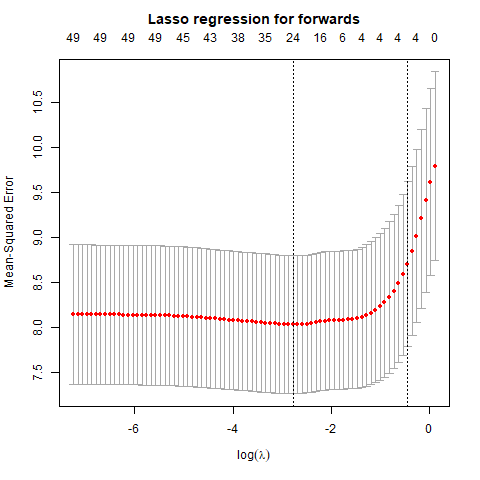
\includegraphics[scale=0.4]{fig/chapter_6/lasso_FWD.png}
    \end{figure}
    \captionof{figure}{RMSE for different values of $\lambda$ for forwards}
    \label{fig:lasso_FWD_1}
\end{minipage}%
\begin{minipage}{.5\textwidth}
  \centering
  \captionsetup{justification=centering}
    \begin{tabular}{c}
    \textbf{Significant variables for Forwards}\\
\\
\\    
\\
\\
Opponent                              \\
Team                                  \\
Cost                                  \\
Transfers in                          \\
Home/Away                             \\
Minutes played                        \\
Goals                                 \\
\\
\\
\\
\\
\\
\\
\\

 \end{tabular}
\captionof{table}{Significant Variables for forwards based on lasso regression and RMSE}
\label{tab:sig_var_FWD_1}
\end{minipage}
\end{table}

\begin{comment}

\begin{figure}[H]
    \centering
    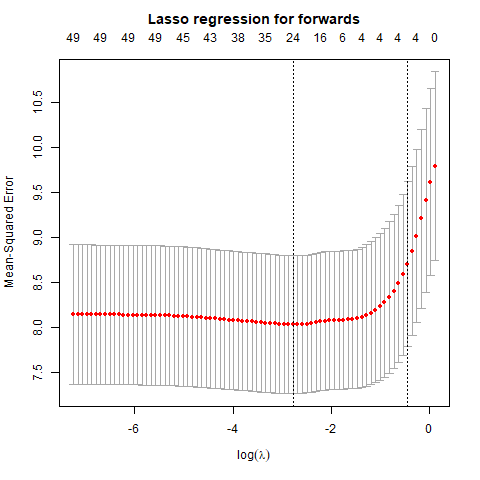
\includegraphics[scale=0.55]{fig/chapter_6/lasso_FWD.png}
    \caption{RMSE for different values of $\lambda$ for forwards}
\label{fig:lasso_FWD}    
\end{figure}

\begin{table}[H]
\centering
\caption{Significant Variables for forwards based on lasso regression and RMSE}
\label{tab:sig_var_FWD}
\begin{tabular}{l}
\textbf{Significant variables for Forwards}\\
Opponent                              \\
Team                                  \\
Cost                                  \\
Transfers in                          \\
Home/Away                             \\
Minutes played                        \\
Goals

\end{tabular}
\end{table}

\end{comment}

\subsubsection{Model Selection}

For each position, a linear regression model is fitted based on the variables. A summmary of each model is presented and a discussion of the signs of the constants is given. It is important to note that the model is continually "refitted" as new data becomes available. That is, the $\beta $s are updated. The variables remain the same. \newpar

\subsection{Odds}
In order to obtain necessary data, we have cooperated with Sportradar, a Norwegian company providing data for bookmakers. Sportradar delivers odds and probabilities of several sports events, including English Premier League. They have provided us with all the necessary probabilities, including result outcomes for each Premier League match as well as individual player probabilities. These data made all the computational work a lot easier, as Sportradar exported structured excel files containing all the necessary data. 
\newpar
Compared to the other two solution approaches, the player list is limited when calculating expected points using odds probabilities. The data from Sportradar was delivered post-season, which has affected the player list. Players that has been transferred or lend to other clubs during the 2017/2018 season are not considered. This is due to the fact that these players are no longer listed in Sportradar's database of Premier League players. In general, the reduced player list will not affect the results of the model, as the players that are lend out are typically lend to clubs in the English Championship division. Hence, these players were not consider good enough to contribute for the teams in the Premier League. However, some of the transfers might have an impact on the results. For instance, players like Philippe Coutinho and Michy Batshuayi are players that contributed with fantasy points in the first half of the season. Unfortunately, these players are not considered when using the odds approach, which is considered as a drawback of the approach.  
\newpar
As odds are primarily available for fixtures in the near future, in general for the upcoming gameweek, the suggested solution approach using odds is further limited. Hence, the horizon on the optimization model is forced to be one gameweek. Compared to the other suggested methods, this is considered a great drawback.

\subsection{Game Chips}
Examining the fixtures list of this year's Premier League season, the game chips are played according to the solution approach suggested in section \ref{Ch.5_Game_chips}. As for the first wildcard, our model is given the opportunity to play it in gameweek 9, where it can either choose to play it or to disregard it for the first half of the season. Hence, the model is not given the opportunity to play the first wildcard in any other gameweeks than in gameweek 9. Further, the triple captain chip can only be played in gameweek 22, as this is the fist double gameweek of the season. Moreover, we allow the bench boost to be played in the second double gameweek of the season, gameweek 34. Hence, the model is given the opportunity to play the second wildcard in gameweek 33, preparing for the bench boost in the following gameweek. As we chose to play the bench boost in the double gameweek 34, we have chosen to allow the model to play a free hit in gameweek 31. This is a blank gameweek, were only 8 team are featured.


\section{Expected Value/Variance trade-off}

\subsection{Variance in the proposed model}

In order to estimate the variance of each player and the correlation between players, their historical performances are considered. In order to obtain somewhat reliable estimations, data for the entire 2016/2017 season is used. Therefore, it is impossible to also find on optimal variance threshold using data on the 2016/2017 season. As a consequence, we have decided not to include expected value/variance trade-off in our proposed model. Instead, the effect of applying the constaint to out solution is described in Section ? and can provide a basis for future research and models-

\subsection{Variance Estimation}
The variance is calculated as the empirical variance in points obtained for each individual player. All previous available data from the 2016/2017 and the 2017/2018 season are used. That is, for gameweek 10 of the 2017/2018, data from all rounds of the 2016/2017 as well as the first nine round of the 2017/2018 season is used.\newpar

\subsubsection{Special cases}
\textit{Lack of historical data}\newline
As previously discussed, complete historical data will not be available for all players for reasons such as promotion or transfers. If only one data-point is available for a player (i.e he has only played one match), it is impossible to calculate his variance. In these cases, the variance is set equal to the average variance of all other players. It is worth noting that this will only be an issue for one match, as more than one data-point will exist afterwards. The lack of data-points are obviously a limitation of the accuracy of the variance estimation, and constitutes a significant source of uncertainty. As the variance trade-off is considered a mean to reduce overall risk, another approach/improvement might consider only picking players with a history of say 10 matches. \newpar

\textit{Zero Variance}\newline
Some players have never played, but can be selected. These players might be interesting to choose for instance in order to fulfill the budget/number of players constraints. However, their empirical variance would equal 0. This is not desirable, as the future performance is not deterministic (they are \textit{not} analogous the the risk-free asset in a portfolio optimization setting). Therefore, their variance is set equal the lowest non-zero variance obtained by other players.

\subsection{Correlation Estimation}

In order to determine the correlation between two players on the same or opposing teams, historical data for the 2016/2017 season is considered. Note that data is aggregated such that only the correlation coefficient between different positions overall is considered. It is not calculated between individual players or teams. Therefore, the correlation between players in the same position in the same team is set equal to 1. In order to determine if a correlation coefficient is significantly different from 0, a hypothesis test is performed. The correlation between players that are not on the same team, nor facing each other in a game-week, is assumed to be 0.\newpar

Table \ref{tab:cor_team} and Table \ref{tab:cor_opp} show the correlation coefficient between different positions as well as the p-value from a hypothesis test with alternative hypothesis of a correlation not equal to 0, for players of the same and opposing teams respectively. In the cases where the correlation is not significant (GLK FWD and DEF FWD of the same teams and GLK GLK of opposing teams), the correlation coefficient is set equal to 0. For the rest, the correlation coefficients ($\rho$) presented in the tables are used.

\begin{table}[H]
\centering
\caption{Correlation coefficient $\rho$ and p-value from significance test for the correlation between players of the same team}
\label{tab:cor_team}
\begin{tabular}{llll}
Position & Position & $\rho$    & p-value  \\
GLK      & DEF      & 0.689  & 2.20 E-16 \\
GLK      & MID      & 0.274  & 1.24 E-10 \\
GLK      & FWD      & 0.0288 & 0.519    \\
DEF      & MID      & 0.368  & 2.20 E-16 \\
DEF      & FWD      & 0.0578 & 0.176    \\
MID      & FWD      & 0.238  & 1.72 E-08
\end{tabular}
\end{table}

\begin{table}[H]
\centering
\caption{Correlation coefficient $\rho$ and p-value from significance test for the correlation between players of opposing teams}
\label{tab:cor_opp}
\begin{tabular}{llll}
Position & Position & $\rho$    & p-value  \\
GLK      & GLK      & 0.0162 & 0.759    \\
GLK      & DEF      & -0.106 & 0.0374   \\
GLK      & MID      & -0.312 & 2.78E-10 \\
GLK      & FWD      & -0.336 & 3.85E-16 \\
DEF      & DEF      & -0.319 & 2.35E-11 \\
DEF      & MID      & -0.447 & 2.20E-16 \\
DEF      & FWD      & -0.292 & 3.35E-09 \\
MID      & MID      & -0.254 & 1.00E-07 \\
MID      & FWD      & -0.136 & 0.00632 \\
FWD      & FWD      & -0.119 & 0.0218  
\end{tabular}
\end{table}